% mnras_template.tex
%
% LaTeX template for creating an MNRAS paper
%
% v3.0 released 14 May 2015
% (version numbers match those of mnras.cls)
%
% Copyright (C) Royal Astronomical Society 2015
% Authors:
% Keith T. Smith (Royal Astronomical Society)

% Change log
%
% v3.0 May 2015
%    Renamed to match the new package name
%    Version number matches mnras.cls
%    A few minor tweaks to wording
% v1.0 September 2013
%    Beta testing only - never publicly released
%    First version: a simple (ish) template for creating an MNRAS paper

%%%%%%%%%%%%%%%%%%%%%%%%%%%%%%%%%%%%%%%%%%%%%%%%%%
% Basic setup. Most papers should leave these options alone.
\documentclass[a4paper,fleqn,usenatbib]{mnras}

% MNRAS is set in Times font. If you don't have this installed (most LaTeX
% installations will be fine) or prefer the old Computer Modern fonts, comment
% out the following line
\usepackage{newtxtext,newtxmath}
% Depending on your LaTeX fonts installation, you might get better results with one of these:
%\usepackage{mathptmx}
%\usepackage{txfonts}

% Use vector fonts, so it zooms properly in on-screen viewing software
% Don't change these lines unless you know what you are doing
\usepackage[T1]{fontenc}
\usepackage{ae,aecompl}


%%%%% AUTHORS - PLACE YOUR OWN PACKAGES HERE %%%%%
% \usepackage(graphicx,tabularx}

% Only include extra packages if you really need them. Common packages are:
\usepackage{graphicx}	% Including figure files
\usepackage{amsmath}	% Advanced maths commands
\usepackage{amssymb}	% Extra maths symbols

%%%%%%%%%%%%%%%%%%%%%%%%%%%%%%%%%%%%%%%%%%%%%%%%%%

%%%%% AUTHORS - PLACE YOUR OWN COMMANDS HERE %%%%%

% Please keep new commands to a minimum, and use \newcommand not \def to avoid
% overwriting existing commands. Example:
%\newcommand{\pcm}{\,cm$^{-2}$}	% per cm-squared

%%%%%%%%%%%%%%%%%%%%%%%%%%%%%%%%%%%%%%%%%%%%%%%%%%

%%%%%%%%%%%%%%%%%%% TITLE PAGE %%%%%%%%%%%%%%%%%%%

% Title of the paper, and the short title which is used in the headers.
% Keep the title short and informative.
\title[Richard Ashley - PhD project]{PhD Progress report - Richard Ashley}

% The list of authors, and the short list which is used in the headers.
% If you need two or more lines of authors, add an extra line using \newauthor
\author[R.P. Ashley et al.]{
R.P. Ashley$^{1}$\thanks{E-mail: r.p.ashley@warwick.ac.uk}\\
% List of institutions
$^{1}$Department of Physics, University of Warwick, Gibbet Hill Road, Coventry, CV4 7AL, UK\\
}

% These dates will be filled out by the publisher
\date{12 August 2015}

% Enter the current year, for the copyright statements etc.
\pubyear{2015}

% Don't change these lines
\begin{document}
\label{firstpage}
\pagerange{\pageref{firstpage}--\pageref{lastpage}}
\maketitle


%%%%%%%%%%%%%%%%%%%%%%%%%%%%%%%%%%%%%%%%%%%%%%%%%%

%%%%%%%%%%%%%%%%% BODY OF PAPER %%%%%%%%%%%%%%%%%%

\section{Outline of the project}
Recent large scale synoptic surveys such as the Catalina Real-time Transit Survey (CRTS), \citep{Drake2009} and the ASAS-SN survey, \citep{ASASSN2014} have yielded a large number of newly discovered transient objects. Many of these objects are compact binaries that exhibit transient phenomena due to the nature of the interaction of the components of the binary. This list includes cataclysmic variable stars that undergo outbursts, binaries that eclipse and pairs of stars that show modulation in their light-curves due to their orbit around each other. Understanding the evolution of these objects benefits from having a large population sample such that the broader statistics of the overall population can be modelled. This is used to place constraints on masses of the components, orbital mechanics and the relative time spent in each phase of the evolution of these systems. Objects detected in these large-scale surveys need to be studied in more detail through having their light-curves resolved with a higher time resolution and with more complete coverage than the surveys can provide. Photometric light-curves will reveal eclipses, phased modulations and timing variations and therefore allow the resolution of the orbital parameters of the systems. Although the transient surveys detect these object through their outburst behaviour, it is also important to study these objects once they have returned to a quiescent phase since other characteristics of the system reveal themselves during these phases. 

The University of Warwick has recently acquired a one metre aperture telescope located at the Roque de los Muchachos Observatory, hereafter refered to as the "One-metre". This telescope will be used to follow up new transient objects detected in current surveys such as, but not limited to, ASAS-SN and CRTS. Since the telescope is not fully commissioned at the moment, a large portion of the PhD project will be the undertaking of the commissioning of the telescope including creation of the software required to operate the telescope remotely and robotically. 


\section{Compact binaries as optical transients}

\subsection{Cataclysmic Variables}
Cataclysmic variables (CVs) are a common state of evolved com- pact binary systems. Such systems consist of a main-sequence, sub- giant or brown dwarf star that is filling its Roche lobe and transfer- ring mass onto a white dwarf \citep{WarnerBook}. The accretion process can be either directly onto a strongly magnetic white dwarf or by way of an intervening accretion disc. 

The study of CVs is an active area of research that can benefit from transient surveys such as CRTS and ASAS-SN. \citet{Breedt2014} use the catalogue to detect and investigate the population of CVs detected as transients in the survey. Understanding a broader population of these objects enables the study of binary evolution of systems like this.  During the lifetime of the CV the orbital period is expected to evolve. Since the orbital period is the most easily observable property of the system, it provides an important indicator to our understanding of the evolution of the system. We cannot usually observe the period changing on human timescales of tens of years so we need a larger population sample that can give us an overview of the various stages of the evolution of the orbit. The orbits of CVs evolve from a long period (several hours) down to a period minimum of about 80 minutes. At this point the donor star will have lost enough mass such that it no longer contains enough to continue hydrogen burning at its core. The thermal timescale of the donor star, which describes how quickly its radius will contract in response to the mass loss, becomes longer than the mass loss timescale itself and the star expands beyond the Roche lobe. Now the dynamics of the system force the separation of the two stars to increase and therefore, in turn, the period also increases. As the system approaches this period minimum, the accretion rate slows down, events take longer and therefore, in a large population sample, we would expect a build-up of systems with periods at around 80 minutes. The period spike has only fairly recently been confirmed from analysis by \citet{Gaensicke2009} of the CVs found in the Sloan Digital Sky Survey (SDSS).  G{\"a}nsicke selected the CV sample through inspection of the spectra taken as part of the SDSS programme. 

Surveys like CRTS that detect objects through optical variability can be used to find CVs \citep{Breedt2014}. Since the cadence of observations for these surveys is much longer than a typical CV orbit, it is not likely that alerts will be generated for CVs that are varying in brightness due to their orbital cycle alone. Detections of CVs have mainly relied on the fact that CVs can dramatically increase in brightness from time to time. Also known as a dwarf novae, a CV in outburst is one in which the accretion disc is undergoing a temporary thermal instability. As the disc becomes more viscous, thermal energy is radiated across its surface. The overall brightness of the system increases by 2 - 6 magnitudes, which corresponds to an increase of from 6 to 250 times its output in quiescence.  The onset of outburst occurs on the timescale of around one day and the outburst itself can last several days or weeks. CVs selected through photometric variability will suffer from a selection bias since those with more frequent outbursts are more likely to be discovered. CVs close to the period minimum are slower accretors and therefore less likely to go into outburst. Slow accretors are known as WZ Sge stars. Since the CRTS survey has been in operation for $\sim 9$ years it is more likely that it is able to detect objects with longer outburst periods and this will improve over the course of the next several years. By following up on CVs detected in CRTS and determining their orbital periods we should be able to find the period spike provided that we carefully take into account the selection affects of these transient detection techniques. If we manage to follow-up on a detection rapidly, we can catch the CV while it is still in outburst and this will allow us to observe it while it is still bright enough to be seen with smaller aperture telescopes, such as the One-metre. We can't expect to observe all of these with such a small aperture, but we can also use other observing programmes that the University of Warwick participates in, such as observations with ULTRACAM on the 4.2m William Herschel Telescope and 3.6m New Technology Telescope and ULTRASPEC observations with the 2.5m Thai National Telescope. 

Some outburst events last for longer than others, maybe a week or more, rather than just a few days. These events are known as super-outbursts. During super-outbursts a phenomenon called a superhump can occur. Here the disc forms an assymetrical component during the outburst and this precesses around the system with a period that is slightly different to the orbital period. Since these phenomena are transient in nature it is useful to be able to follow up on the detection of an outburst within a day or so, while the superhump is still evident. If an outburst is detected by one of the transient surveys than we can schedule observations on the One-metre as a follow up. 

\subsection{Polars}
CVs that include white dwarf stars with strong magnetic fields define a sub-class known as polars, \citep{CropperReview}. Polars are so-called because the optical radiation coming from the object is strongly polarised. In most CVs the matter accreting from the donor star is expected to form an accretion disc around the white dwarf but this does not happen in Polars. Since the accretion stream is composed of hot hydrogen gas in free fall that is heating up to beyond ionisation temperature, it becomes a plasma that can be affected by magnetic fields. Therefore, if the white dwarf's magnetic field is strong enough, it can divert the flow of the stream such that it now follows the field lines and, rather than forming a disc in the plane of the CV's orbit, the stream diverts to accrete directly on to one or both of the CVs magnetic poles. Since polars do not have a disc, they are not able to go into outburst as dwarf novae. Most polars do however have different states of activity, corresponding to higher or lower accretion rates. Polars can also show intermediate states where the accretion rate is somewhere between the highest and lowest. The brightness variation between these two states varies from system to system and may be correlated to the orbital period \citep{WarnerBook}, with a maximum variation of about 5 magnitudes (100 times).

Surveys like CRTS have already been fruitful in finding new polars by detecting their high-state versus low-state variability. 

\section{Optical transient surveys}

\subsection{Catalina Real Time Survey}
The original and primary purpose of progenitor to CRTS, the Catalina Sky Survey, was to detect near-Earth objects such as asteriods that are of interest to solar system astronomers and could be important for an early warning of any objects on a potential collision course with Earth. More generally, the survey is being used to identify many kinds of optical transients that vary on timescales from minutes to years. The most recent catalogue of identified transients can be found in \citet{CatalinaCatalog}. So far, CRTS has detected more than 9000 transient objects since its start of operations in 2007. The survey makes use of a network of  small telescope situated in 3 locations around the world, two in the USA and one in Australia. The survey covers an area of the sky of $\sim 30,000\,deg^2$ between $-75^\circ < \delta < 65^\circ$ excluding an area of a few degrees near the galactic plane and revisits most locations many times per year with a typical cadence of around 2 weeks. The limiting magnitude of the survey is about $19-21$, depending on the telescope. Details of the telescopes and the observing program are described in \citet{Drake2009}. 

Since the survey has been in operation for $\sim 9$ years, it is growing in utility for detecting rarer transient events. An example of these types of events is a dwarf novae outburst. These events can occur on times scales of a few weeks, but are understood to also happen only over the course of dozens of years. Detecting these events and following up with optical photometry is important in understanding comapct binary evolution. This topic is discussed in more detail in the next section of this report. 

\subsection{GAIA}
The GAIA satellite was launched in 2013. Over the course of the next five or so years, it will measure the position and magnitude of around 1 billion stars with about 70 separate measurements each. This will provide a large source of optical transients. Detected transients are published via a system called the GAIA alerts system \footnote{\url{http://www.gaia.ac.uk/selected-gaia-science-alerts}}. This system will provide a live source of objects that might be compact binaries and worthy of follow up in this project. An aim of this PhD project is to implement a GAIA allerts follow up service with the newly commissioned One-metre telescope.  At the moment, these alerts are not live, but are expected to come online in November 2015. The time delay from object detection to the public release of the alert is undefined as the identification pipeline is still in development. The expectation is that, once the pipeline is established, alerts will be released in near real-time (minutes to hours) after detection. The One-metre telescope will then add any relevant alerts to its own observing schedule.  

\subsection{ASAS-SN}
The "All-Sky Automated Survey for Supernovae" (ASAS-SN or "Assassin") project, will eventually automatically survey the entire visible sky every night down to about 17th magnitude. Although its primary purpose is the search for new supernovae, it detects many transients.  Bright transients, Galactic and extragalactic, discovered early by our high-cadence survey, are especially valuable, as they are easy to study using relatively modest size telescopes.

ASAS-SN is currently comprised of two units. ASAS-SN Unit-1, known as "Brutus", is comprised of four robotic 14-cm telescopes located at the Haleakala station of the Las Cumbres Observatory Global Telescope Network (LCOGT). ASAS-SN Unit-2, named "Cassius", also consists of four 14-cm telescopes deployed at the LCOGT Cerro Tololo station. Together, these observe a total of approximately 20,000 square degrees on each night. Overall the survey covers the whole sky, although the position of the sun and the moon mean that not all of the sky is covered throughout the year. 

ASAS-SN is already providing a rich feed of newly discovered cataclysmic variables for follow up observations. Since April 2013 ASAS-SN has identified over 180 new cataclysmic variable stars and announced over 260 new outbursts of known CVs, \citep{Davis2015}. Recently, the ASAS-SN project has launched an online tool to provide an active feed of CVs displaying outbursts, known as CV Patrol\footnote{\url{http://cv.asassn.astronomy.ohio-state.edu/}}.  During the course of this PhD project, this service will be incorporated as part of the input for finding new populations of compact binaries to study.  

\section{Current Progress}

\subsection{One-metre Telescope}
The One-metre telescope (Fig. \ref{fig:telescope}) is situated on the island of La Palma at the Roque de los Muchachos observatory. At the start of the project, in January 2015, the telescope was installed in the dome, but not operational. The major factors in its status were instrument readiness, the software stack and image quality. In this section we will describe each area in more detail. 

The One-metre telescope was originally commissioned by Don Pollaco, in collaboration with several other academics at various institutions, in order to act as a follow up to the exoplanet candidates detected in the SuperWASP \citep{PollaccoSuperWASP} survey. Objects cataloged in SuperWASP need to be followed up by another telescope in order to confirm that they are genuine exoplanet transits and to better determine parameters such as transit depths and orbital periods. The design of the One-metre includes a camera that is able to make simultaneous measurements in two colours. Using two colours helps to disambiguate other affects from a transit detection. For example, a background star might be causing a false positive affect for a transit, but it is generally true that changes due to another stellar object will vary in each different colour band, whereas a planetary transit (at first approximation) is expected to be `grey' or equal in all colours. Stellar activity of the host star is likely to by larger in one colour than another and so any changes due to variations in the star's intrinsic output will be different in each of the colour bands and can therefore be ruled out by simultaneous two-colour observations. Now that the scope of the telescope's scientific work has been expanded to include the observation of compact binary objects and other transients with white dwarf components, it needs to be adapted to take photometric observations at bluer wavelengths. 

\subsubsection{Image Quality}
Tests in March 2015 showed that the telescope was able to take images, but suffered from some poor image quality artifacts. There was a significant coma around stars when in focus and a very pronounced non-circular artifact when out of focus. Fig. \ref{fig:coma} shows the comas when imaging the moons of Jupiter and Fig. \ref{fig:ellipse} shows the image artifact when taking the telescope out of focus, through focus and then out of focus again. Research into telescope optics suggested that, since the out-of-focus image artifact shift through $90^\circ$ when going through focus, that it was caused by `pinching'. Pinching is caused by distortion of the primary mirror which, in turn, can be caused by mechanical pressure on the mirror. As can be seen in Fig. \ref{fig:telescope} there is a large baffle attached to the primary mirror. When this was removed, it was found to weigh approximately 14 kg and that its mounting point is in direct contact with the primary mirror. Without the baffle in place, the image quality improved significantly, as shown in Fig. \ref{fig:ellipse-corrected}. During a subsequent site visit, the collimation of the primary and secondary mirrors was adjusted to improve the image quality even further. At the moment, the workshop at the University of Warwick is constructing a new lightweight version of the baffle and this is due to be installed on the telescope by October 2015. At this point further tests into the image quality will be carried out.  

% Telescope
\begin{figure}
	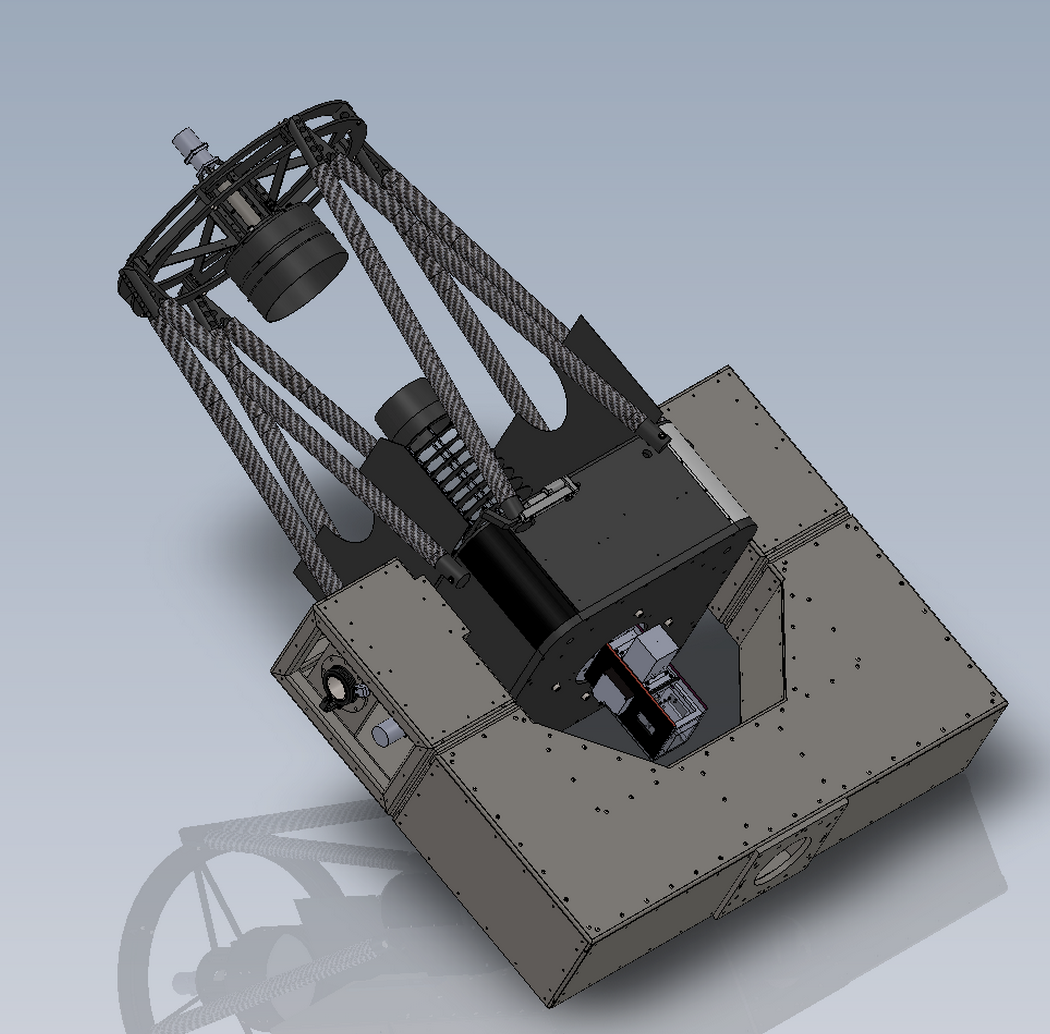
\includegraphics[width=\columnwidth]{images/telescope.png}
    \caption{Technical drawing of the One-metre telescope, including the fork that forms part of the equatorial mount.  Note the large baffle mounted on the primary mirror (discussed in the text).}
    \label{fig:telescope}
\end{figure}

% Comas
\begin{figure}
	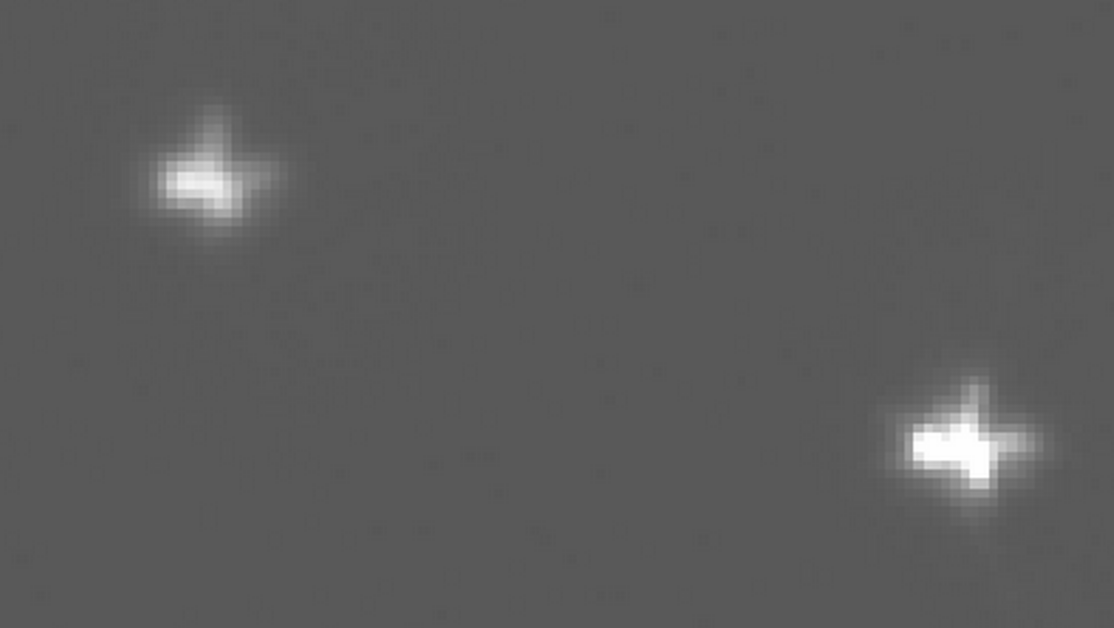
\includegraphics[width=\columnwidth]{images/comas.png}
    \caption{Image of two of Jupiter's moons showing comas.}
    \label{fig:coma}
\end{figure}

% Ellipse
\begin{figure}
	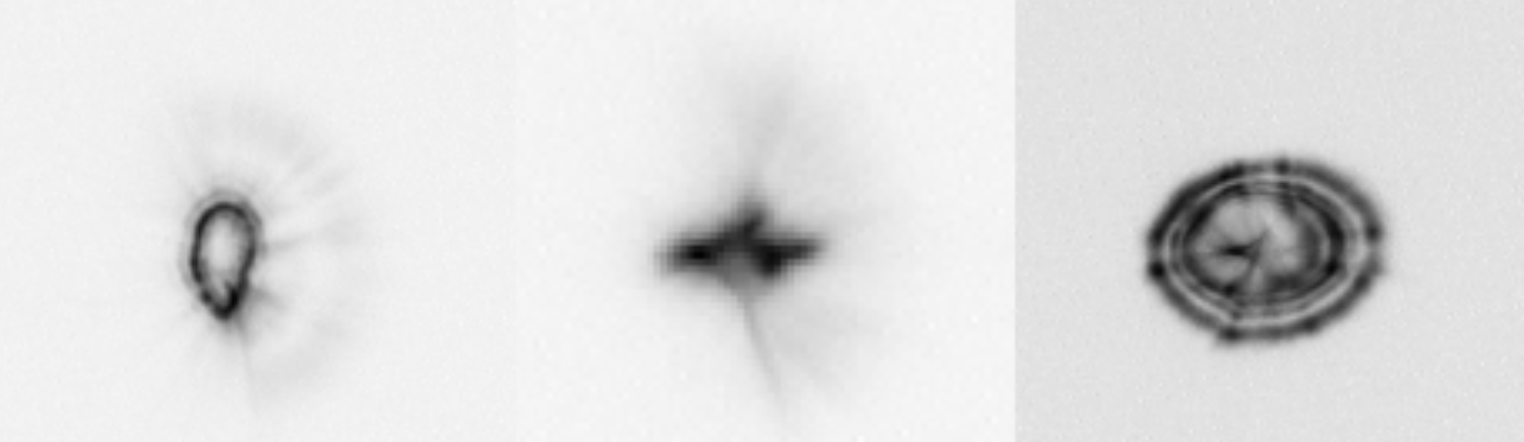
\includegraphics[width=\columnwidth]{images/ellipse.png}
    \caption{Images of a bright star taken on each side of focus with the baffle causing `pinching'.}
    \label{fig:ellipse}
\end{figure}

% Ellipse corrected
\begin{figure}
	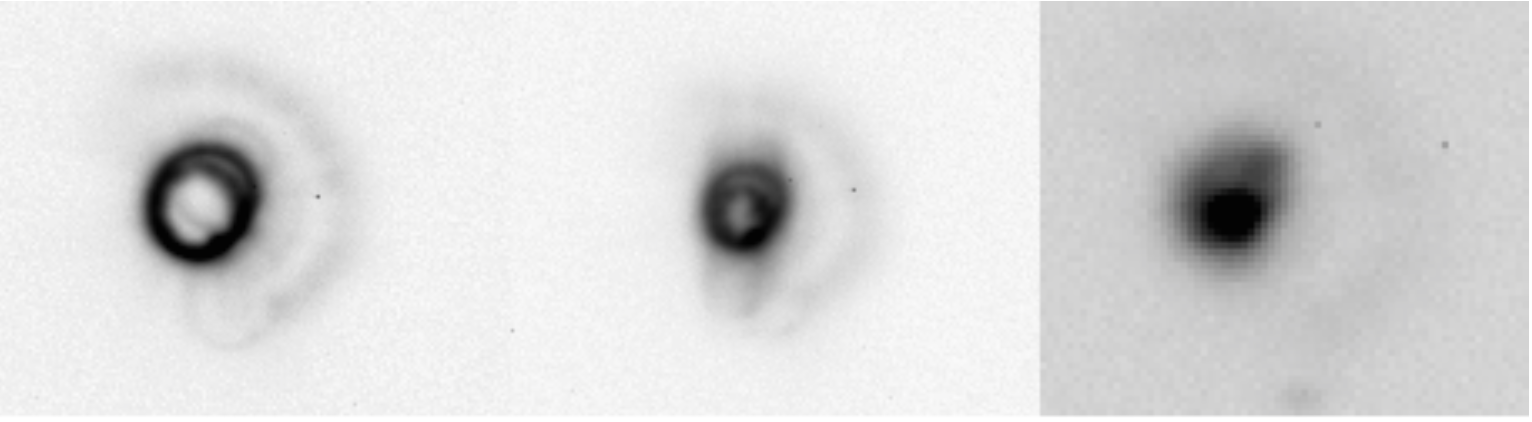
\includegraphics[width=\columnwidth]{images/ellipse-corrected.png}
    \caption{Images of a bright star taken on each side of focus after the baffle has been removed. Note that the elliptical image artifact is no longer present, but the coma remains.}
    \label{fig:ellipse-corrected}
\end{figure}


\subsubsection{Telescope Software}
There are two software utilities that have been installed on the machines in the dome. Talon is the core telescope control software that is provided by the manufacturer of the telescope, Optical Mechanics Incorporated or OMI. In addition to this core driving software, collaborators at the Institut de Ci\`{e}ncies de l'Espai in Barcelona have built and installed a software package called OpenROCS\footnote{\url{http://sourceforge.net/projects/openrocs/}} that will be used to control the overall operation of the complete installation, including the telescope, dome and environmental monitoring. 

Full automation of the telescope will require the development of software to coordinate the environmental monitoring with the dome and telescope, effectively adding logic to OpenROCS. We will also need to develop software that will handle the scheduling and prioritisation of the observing work cycle. None of this software has been written yet, but we are in the process of planning and researching the correct approach. It is expected that we will begin writing the first version of the software in December 2015. 

A fully automated software reduction pipeline is also planned. This will take the raw images produced by the two cameras and perform a full reduction of the objects contained in the field. This will enable the inspection of the science data in near real-time, ie immediately after the science run is completed, or perhaps live previews of the light-curves of the targets during the observations themselves. The pipeline will make use of the existing work done by the author in automating the reduction of the ULTRACAM and ULTRASPEC pipelines, \citep{RashleyMSC}. Although we plan to have an automated pipeline in place, we will also ensure that all raw data from nightly observations is backed up and sent to an archive on the Warwick hosted IT systems. 

\subsubsection{Cameras}
The telescope is intended to use two cameras simultaneously so that it can record photometry in two colour bands. It has already been fitted with two Andor Ikon-L series cameras. One camera is designated for the 'blue' channel and the other the 'red' channel. The red camera uses a deep-depleted CCD and 5-stage Peltier cooler to improve the NIR sensitivity. Typically it is cooled to about $-90^\circ C$. The 'blue' camera is also Peltier cooled, but is cooled to a temperature of about $-70^\circ C$.  

The optical path of the camera is laid out such that light coming from the secondary, through the Cassegrain aperture, first encounters a dichroic filter, angled at $45^\circ$, that reflects the blue component to the blue camera, mounted at $90^\circ$ to the optical axis and allows the red light to pass through to the red camera on the optical axis. 

In March 2015 the team working on the telescope, Paul Chote and the author, made a trip to La Palma to begin the process of commissioning. It was discovered that one of the cameras was not responding to communication requests from the data acquisition computer. This was eventually traced to a faulty communication cable. Although the cable has been replaced, the camera is still not ready for operation as it needs a firmware upgrade. This is planned for August 2015. Once the red camera's firmware is upgraded, both cameras will be returned to the telescope and be ready for operation. 

\subsubsection{Filters}
When the telescope was originally commissioned, the filters provided were chosen to optimise the data gathered for exoplanet transits as described above. The filters originally installed were the SDSS z filter and the RISE-1 filter. However, since we now want to observe bluer targets, we are proposing to alter the filter set. The SDDS z filter will remain in place, but we will switch the RISE-1 filter for a broad blue pass-band filter such as the BG40. If we encounter problems in sourcing this filter there are alternatives, such as the KG5. We will also need to replace the dichroic to ensure that we have the correct split of light down each optical path.  The original and proposed filters, along with the camera quantum efficiencies are shown in Fig. \ref{fig:filters}.

% Filter plots
\begin{figure}
	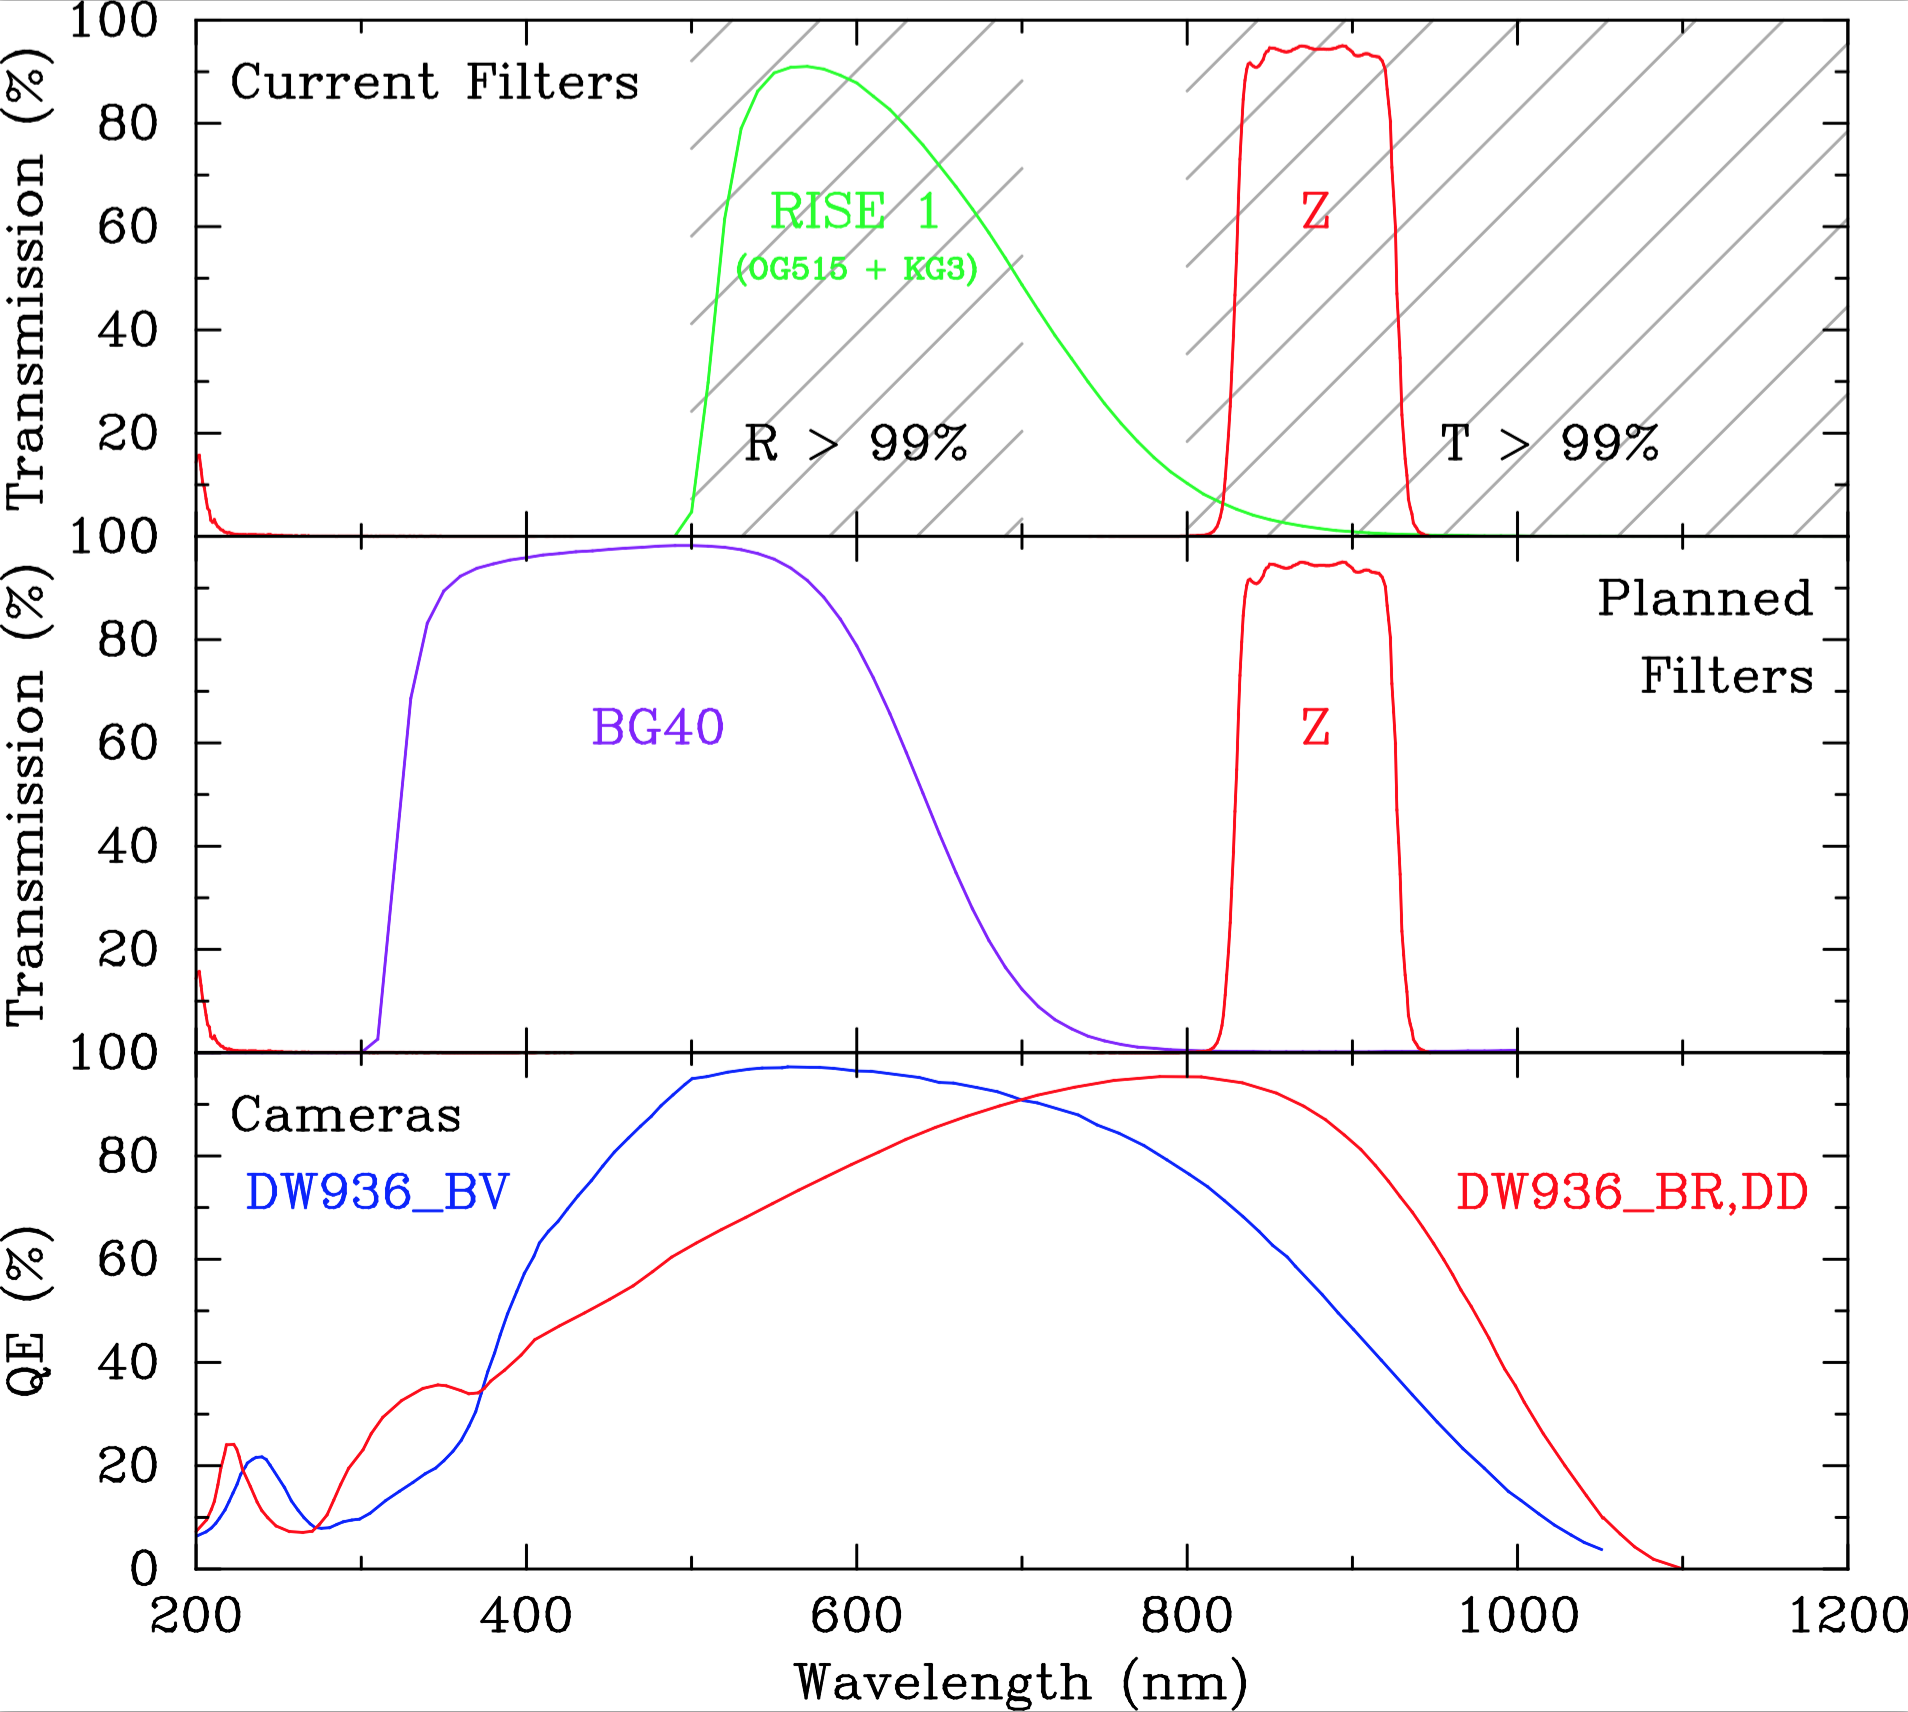
\includegraphics[width=\columnwidth]{images/filters.png}
    \caption{The original and the newly proposed filter set for the One-metre telescope. The upper panel shows the current filter set (as of July 2015) with the hashed region indicating where the dichroic splits the light for each optical path. The middle panel shows the proposed new blue filter. The lower panel shows the quantum efficiency curves of the two cameras. }
    \label{fig:filters}
\end{figure}

Since there are still many tasks to perform in getting the telescope control software operational, the new filter and dichroic have not been ordered yet. This is planned for later in the year or early 2016, once the telescope itself is operating more smoothly.

\subsubsection{Dome and environment}
The site at La Palma, while being a place of relatively low humidity, can suffer from very high humidity during adverse weather conditions. Visual inspection of items in the dome indicate very clearly that there can be significant amounts of water building up within the enviroment. Ferrous surfaces are all rusted and the primary mirror shows signs of stain due to water collection and evaporation. The project team has ordered and is in the process of fitting several environment monitoring tools. These will allow us to keep track of changing conditions at the telescope and will provide an input to the control software stack for making decisions on when to close or open the dome. Steps to reduce the overall humidity in the dome are also being taken. A large de-humidifier is being ordered and plans to insulate the floor of the telescope platform are being considered.  

\subsubsection{First light}
During the excursion to the telescope in March 2015, although images were taken with the red camera of the telescope, it was not possible to obtain any scientific data. Issues related to the image quality, the lack of operation of the camera and the general state of the telescope itself took higher priority than any need to gather scientific observations. 

In July 2015, on a second visit to the site, a short observation of the pulsating white dwarf known R808. The 14th magnitude pulsator was observed for about 100 minutes at a cadence of 5 seconds. Observations were taken in white light with only the red camera in operation.  The reduced light curve is shown in Fig. \ref{fig:r808} and shows the pulsations quite clearly (with an amplitude of about 20 mmag). This is a very early test of the potential science output of the telescope, but demonstrates that, once our maintenance is complete, science with this telescope will be possible.

% Filter plots
\begin{figure}
	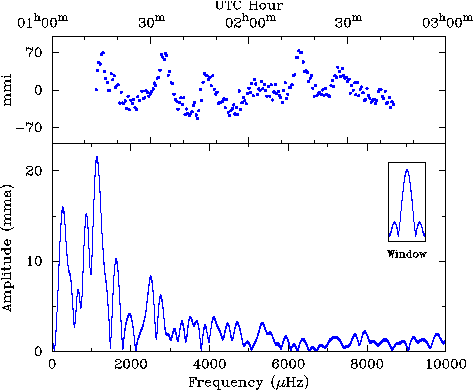
\includegraphics[width=\columnwidth]{images/r808.pdf}
    \caption{The light curve and amplitude spectrum for R808 (a 14th magnitude pulsating White Dwarf (DAV), taken by the One-metre telescope in July 2015.}
    \label{fig:r808}
\end{figure}
 
\subsection{Active research}
In addition to commissioning the One-metre telescope, I am working on publishing new research on polars. In particular, the polar known as CSS081231:071126+440405 (hereafter,  CRTS\,J0711+4404), which was discovered in the CRTS survey when it went into a high state in 2008.  CRTS\,J0711+4404 is an eclipsing polar that shows  clear, sharply defined eclipses  with a period of 117 minutes caused when the primary (white dwarf), the accretion stream and the accretion spot all disappear behind the secondary mDwarf.  \citet{Schwope2015} and \citet{Worpel2015} have published findings based on photometry, spectroscopy and X-ray observations of the polar. Schwope used photometry taken from various telescopes over the past 7 years to define the orbital parameters of the system and to set mass contraints on any potential orbiting planet. He determined the inclination of the system and computed a linear ephemeris for the eclipses. Schwope suggested that there may be accretion on to both poles of the white dwarf as shown by a tentative detection of a small increase in brightness of the system at phase 0.5. Schwope also comments on the occasional appearance of a pre-eclipse dip at phase 0.75. This is thought to be due to the accretion curtain eclipsing the bright accretion spot.  

\citet{Worpel2015} use XMM-Newton observations to show that CRTS\,J0711+4404 does indeed appear to be accreting onto both poles. The X-ray spectrum shows that the hot thermal component of the accreting plasma is at a temperature of a few tens of $keV$ with the blackbody spectrum of the heated region of the white dwarf has a temperature of $50-100 eV$. Worpel also fits cyclotron models to an optical spectrum taken at phase 0.18 to determine a field strength of $36MG$. 

We have three key sets of observations of CRTS\,J0711+4404 that will allow us to make further conclusions about the system. These are a set of photometry taken at the Thai National Telescope using the ULTRASPEC instrument and two sets of time resolved optical spectra with one set taken during the low state of the polar and the other set taken during high state. Both sets of spectra were taken with the ISIS dual-beam spectrograph on the William Herschel Telescope in La Palma.

The high speed photometry covers 7 eclipses of the system taken on 6 separate nights in 2014 and 2015. These observations are the highest cadence and signal-to-noise of any photometric observations taken so far. This has allowed us to compute a refined ephemeris for the system. Our photometry does not show any obvious sign of a pre-eclipse dip which is noteworthy. Measuring the precise timing and phase of the accretion stream relative to the eclipse will allow us to make an estimate of the accretion geometry. The geometry might be subject to changes as the polar goes from low state to high state with material accreting onto a slightly different spot near the magnetic pole when the accretion switches. Since our observations were all taken in high state, it will be valuable to compare these observations to those of Schwope which cover a combination of low and high states. 

In February 2009, 17 spectra were taken of the target in low state. These observations cover phases 0.64 through to 1.32 and include a spectrum taken entirely during the eclipse of the white dwarf and the accretion stream. This means that we have a measurement mDwarf spectrum without contamination from other components in the system. By subtracting this spectrum from spectra taken at other phases of the orbit, we can see the evolution of the spectral features of the white dwarf and accretion stream as the orientation changes. Fitting cyclotron models to these spectra allows us to follow the angle of orientation of the stream to the observer. In many of the spectra, the sodium NaI doublet at $8190 \AA$ is clearly visible. By fitting a double gaussian to this feature for each spectrum we are able to compute the radial velocity variation through the orbital cycle. This feature is tied to the photosphere of the mDwarf donor star and our fit gives us the orbital velocity, or $K_2$ semi-amplitude of the system. 

With our additional data, we will be able to publish new findings on this object, such as new estimates for the masses of the components, the temperature of the accretion plasma and the strength of the magnetic field. We will also be able to confirm observations made by Schwope and Worpel. 

A paper for submission to the Monthly Notices of the Royal Astronomical Society is being prepared and is in draft form at the moment. 

\subsection{Observing experience}
Since January 2015, I have been on 4 observing runs in Thailand and La Palma. A week long observing run on the Thai National Telescope using ULTRASPEC gave me experience of taking high speed photometry of optical transients. I have also participated in an ULTRACAM run at the William Herschel Telescope at La Palma. This task included unpacking and mounting the instrument on the telescope. 

I have had two spectrographic observing runs on the Isaac Newton Telescope. Both of these runs were solo efforts with me being the only observer at the telescope. The tasks included scheduling, planning and preparing for the run as well as data reduction during the observations. During these runs, the science work was to look for radial velocities in targets that were suspected white dwarf, mDwarf binaries. Several of these targets were confirmed as binaries and follow up observations are planned with observing time allocated.  

From October 2015, I will be working on La Palma as an intern in the Isaac Newton Group of Telescopes (ING) studentship program. This position will allow me to spend 60\% of my time continuing with the PhD research, while 40\% will be dedicated to tasks set by the ING. During this time I will be exposed to many different aspects of observational astronomy, from instrumentation maintenance to scripts for reduction and documentation. I will also have the opportunity to meet many working astronomers from a variety of different research areas and develop a broader vision of the field from them.  Being based on the island for a year will be a large advantage for our work on the One-metre telescope as the rest of the team will be based back at the University of Warwick.  

\section{Conclusions}
This PhD is focused on producing new insights into the population statistics and thereby the understanding of the evolution of compact binary systems. Its goals are a combination of commissioning a new automatic telescope and using it to follow up on transient objects detected in surveys to catalog newly discovered compact binaries. 

The One-metre telescope that forms an important part of this project is in a state that is not yet ready for scientific data gathering, but it is expected that towards the end of 2015 and the start of 2016, the bulk of the urgent maintenance work will be complete and the telescope will be able to commence operation. During 2016, the telescope scheduling and reduction software will be developed and robotic observations should be possible in 2017.

Active research into understanding the nature of compact binary objects is already in progress and a paper for publishing in a reviewed scientific journal is currently in draft.

Work in the latter half of 2016 and all of 2017 will focus on ensuring the One-metre telescope is in operation and able to follow up on transients detected in surveys.


%%%%%%%%%%%%%%%%%%%%%%%%%%%%%%%%%%%%%%%%%%%%%%%%%%

%%%%%%%%%%%%%%%%%%%% REFERENCES %%%%%%%%%%%%%%%%%%

% The best way to enter references is to use BibTeX:

\bibliographystyle{mnras}
\bibliography{../rashley} 


% Alternatively you could enter them by hand, like this:
% This method is tedious and prone to error if you have lots of references
%\begin{thebibliography}{99}
%\bibitem[\protect\citeauthoryear{Author}{2012}]{Author2012}
%Author A.~N., 2013, Journal of Improbable Astronomy, 1, 1
%\bibitem[\protect\citeauthoryear{Others}{2013}]{Others2013}
%Others S., 2012, Journal of Interesting Stuff, 17, 198
%\end{thebibliography}

%%%%%%%%%%%%%%%%%%%%%%%%%%%%%%%%%%%%%%%%%%%%%%%%%%

%%%%%%%%%%%%%%%%% APPENDICES %%%%%%%%%%%%%%%%%%%%%

%\appendix

%\section{Some extra material}

%If you want to present additional material which would interrupt the flow of the main paper,
%it can be placed in an Appendix which appears after the list of references.

%%%%%%%%%%%%%%%%%%%%%%%%%%%%%%%%%%%%%%%%%%%%%%%%%%


% Don't change these lines
\bsp	% typesetting comment
\label{lastpage}
\end{document}

% End of mnras_template.tex
